\documentclass[10pt,letterpaper,extrafontsizes]{memoir}
\listfiles
\usepackage{comment}


% For (non-printing) notes  \PWnote{date}{text}
\newcommand{\PWnote}[2]{} 
\PWnote{2009/04/29}{Added fonttable to the used packages}
\PWnote{2009/08/19}{Made Part I a separate doc (memdesign.tex).}

% same
\newcommand{\LMnote}[2]{} 


\usepackage{memsty}
%%%%%%%%%%%%%%%%%%%%%%%%%%%%
\usepackage{titlepages}  % code of the example titlepages
\usepackage{memlays}     % extra layout diagrams
\usepackage{dpfloat}     % floats on facing pages
\usepackage{fonttable}[2009/04/01]   % font tables
%%%%\usepackage{xr-hyper} \externaldocument{memdesign} Doesn't work, 
%%%%                      Idea won't work in general for memman/memdesign
%%%%                      as at display time, who knows where everything
%%%%                      will be located on the individual's computer.
%%%%%%%%%%%%%%%%%%%%%%%%%%%%

\usepackage{listings}
\usepackage{color}

\definecolor{dkgreen}{rgb}{0,0.6,0}
\definecolor{gray}{rgb}{0.5,0.5,0.5}
\definecolor{mauve}{rgb}{0.58,0,0.82}

\lstset{frame=tb,
  language=C++,
  aboveskip=3mm,
  belowskip=3mm,
  showstringspaces=false,
  columns=flexible,
  basicstyle={\small\ttfamily},
  numbers=none,
  numberstyle=\tiny\color{gray},
  keywordstyle=\color{blue},
  commentstyle=\color{dkgreen},
  stringstyle=\color{mauve},
  breaklines=true,
  breakatwhitespace=true,
  tabsize=3
}
%%%% Change section heading styles
%%%\memmansecheads

%%%% Use the built-in division styling
\headstyles{memman}

%%% ToC down to subsections
\settocdepth{subsection}
%%% Numbering down to subsections as well
\setsecnumdepth{subsection}

%%%% extra index for first lines
\makeindex[lines]


% this 'if' is used to determine whether we are compiling the memoir
% master in the subversion repository, or the public memman.tex
\newif\ifMASTER
\MASTERfalse
%\MASTERtrue

\ifMASTER

% add patch to fink, such that \AtEndFile still work
\makeatletter
\AtEndFile{fink.sty}{
  \typeout{patching fink} 
  \renewcommand{\InputIfFileExists}[2]{%
    \IfFileExists{##1}%
    {##2\@addtofilelist{##1}%
      \m@matbeginf{##1}%
      \fink@prepare{##1}%
      %\@@input \@filef@und
      \expandafter\fink@input%
      \expandafter\fink@restore\expandafter{\finkpath}%
     \m@matendf{##1}%
     \killm@matf{##1}}%
 }
}
\makeatother
% private package, not in circulation
% enables us to gather svn information on a single file basis
%\usepackage[filehooks]{svn-multi-private}
% use the current version
\usepackage[filehooks]{svn-multi}


% \svnidlong
% {}
% {$LastChangedDate: 2015-03-05 18:49:59 +0100 (Thu, 05 Mar 2015) $}
% {$LastChangedRevision: 516 $}
% {$LastChangedBy: daleif $}



\makeatletter
\newcommand\addRevisionData{%
  \begin{picture}(0,0)%
    \put(0,-20){%
      \tiny%
      \expandafter\@ifmtarg\expandafter{\svnfiledate}{}{%
        \textit{\textcolor{darkgray}{Chapter last updated \svnfileyear/\svnfilemonth/\svnfileday
         \enspace (revision \svnfilerev)}}
     }%
    }%
  \end{picture}%
}
\makeatother

% we add this to the first page of each chapter

\makepagestyle{chapter}
\makeoddfoot{chapter}{\addRevisionData}{\thepage}{}
\makeevenfoot{chapter}{\addRevisionData}{\thepage}{}

\else
% disable svn info collecting
\newcommand\svnidlong[4]{}
\fi



%% end preamble
%%%%%%%%%%%%%%%%%%%%%%%%%%%%%%%%%%%%%%%%%%%%%%%%%%%%%%%
%#% extend

\usepackage[draft]{fixme}
\fxsetup{
  layout=marginnote
}
 

\begin{document}




%#% extstart input intro.tex





%\tightlists
\firmlists
\midsloppy
\raggedbottom
\chapterstyle{demo3}

%%%%%%%%%%%%%%%%%%%%%%%%%%%%%%%%%%%%%%%%%%%%%%%%%%%%%%%


\ProvidesFile{memnoidxnum}[2009/04/30  some index entries for memman]
\newcommand*{\idxat}{\index{@?\texttt{@}|noidxnum}} \idxat
%%\index{@?\texttt{@}|noidxnum}
\index{argument|noidxnum}
%%\index{array|noidxnum}
\index{cardinal|noidxnum}
\index{centering|noidxnum}
%%\index{chapterstyle|noidxnum}
%%\index{counter|noidxnum}
\index{default|noidxnum}
\index{division|noidxnum}
\index{division!sectional|seealso{subhead}}
\index{double column|noidxnum}
\index{endnote!mark|seealso{reference mark}}
\index{environment|noidxnum}
\index{error message|noidxnum}
\index{figures|noidxnum}
%%\index{file|noidxnum}
\index{font characteristic|noidxnum}
\index{footnote!mark|seealso{reference mark}}
\index{footnotes|noidxnum}
\index{frame|noidxnum}
\index{framed|noidxnum}
\index{full stop|seealso{period}}
\index{hanging|noidxnum}
\index{headstyles|noidxnum}
%%\index{horizontal|noidxnum}
\index{Hurenkinder|see{widow}}
\index{interlinear space|see{leading}}
\index{keyword|noidxnum}
%%\index{label|noidxnum}
\index{LaTeX?\ltx|noidxnum}
%%\index{length|noidxnum}
\index{line|noidxnum}
\index{line too long|see{overfull lines}}
\index{lining|noidxnum}
%%\index{list|noidxnum}
\index{lowercase|noidxnum}
\index{MakeIndex?\Pmakeindex|noidxnum}
\index{margin!spine|seealso{inner}}
\index{margin!inner|seealso{spine}}
\index{margin!foredge?\foredge|seealso{outer}}
\index{margin!outer|seealso{\foredge}}
\index{margin!upper|seealso{top}}
\index{margin!top|seealso{upper}}
\index{math|noidxnum}
%%\index{memoir class|noidxnum}
\index{minipage|noidxnum}
\index{name|noidxnum}
\index{named|noidxnum}
\index{new|noidxnum}
%%\index{number|noidxnum}
\index{numeric|noidxnum}
\index{old-style|noidxnum}
\index{option|noidxnum}
\index{ordinal|noidxnum}
\index{outline|noidxnum}
\index{package|noidxnum}
\index{page break|noidxnum}
%%\index{pagestyle|noidxnum}
\index{paragraph break|noidxnum}
\index{period|seealso{full stop}}
\index{poem|noidxnum}
\index{program|noidxnum}
\index{ranging|noidxnum}
\index{reference|noidxnum}
\index{reference mark|seealso{endnote mark, footnote mark}}
\index{representation|noidxnum}
\index{rule|noidxnum}
\index{ruled|noidxnum}
%%\index{section|noidxnum}
\index{Schusterjungen|see{orphan}}
\index{section|seealso{subhead}}
\index{sectional division|seealso{subhead}}
\index{single column|noidxnum}
\index{size|noidxnum}
\index{space|noidxnum}
\index{space!double|see(double spacing)}
\index{space!between lines|see{leading}}
\index{stanza|noidxnum}
%%\index{subfloat|noidxnum}
\index{TeX?\tx|noidxnum}
\index{text|noidxnum}
\index{titling|noidxnum}
\index{trim|noidxnum}
%%\index{type size|noidxnum}
\index{vertical|noidxnum}
\index{warning|noidxnum}
\index{write|noidxnum}
%%\index{XeTeX?\xetx|noidxnum}

%%%%%%%% Deleted the font indexing (now done as typefaces) 2009/04/30

\begin{comment}
\index{table of contents|see{ToC}}
\index{list!of figures|see{LoF}}
\index{figure!list of|see{LoF}}
\index{list!of tables|see{LoT}}
\index{table!list of|see{LoT}}
\index{marginal note|see{marginalia}}
\index{footnote!in title|see{thanks}}
\index{illustration|seealso{float, figure}}
\index{figure|seealso{float}}
\index{table|seealso{float}}
\index{chapter!style|see{chapterstyle}}
\index{chapter!heading|see{heading}}
\index{page!style|see{pagestyle}}
\index{part!heading|see{heading}}
\end{comment}

\begin{comment}

%%%% deleted the \nocites
%
\index{anonymous division|see{division}}
\index{array|seealso{tabular}}
%
\index{Berne Convention|see{copyright}}
\index{blank page|see{page}}
\index{Buenes Aires Convention|see{copyright}}
\index{box!rule|seealso{rule}}
%
\index{chapter|seealso{division}}
\index{chapter!style|see{chapterstyle}}
\index{command|seealso{declaration, macro}}
\index{comptexttex?\texttt{comp.text.tex} newsgroup|see{\ctt}}
\index{Comprehensive TeX Archive Network?\cTeXan|see{\ctan}}
\index{contents list|see{ToC}}
\index{counter representation!Alph tt?\texttt{Alph}|see{\texttt{Alph}}}
\index{counter representation!alph tt?\texttt{alph}|see{\texttt{alph}}}
\index{counter representation!arabic tt?\texttt{arabic}|see{\texttt{arabic}}}
\index{counter representation!Roman tt?\texttt{Roman}|see{\texttt{Roman}}}
\index{counter representation!roman tt?\texttt{roman}|see{\texttt{roman}}}
\index{counter representation!fnsymbol tt?\texttt{fnsymbol}|see{\texttt{fnsymbol}}}
\index{cross reference|seealso{reference}}
%
\index{descriptive list|see{list}}
\index{display math|see{math}}
\index{display mode|see{display}}
\index{division|seealso{heading}}
%
\index{electronic book|see{ebook}}
\index{enumerated list|see{list}}
%
\index{figure!list of|see{LoF}}
\index{figure|seealso{float}}
\index{float!numbered captioning|see{caption}}
\index{float!unnumbered captioning|see{legend}}
\index{font characteristic!weight|see{series}}
%
\index{file|seealso{stream}}
\index{footnote!in title|see{thanks}}
\index{fragile command|seealso{protect}}
\index{free tabular|seealso{tabular}}
%
\index{header|seealso{running header}}
\index{heading|seealso{division}}
%
\index{illustration|seealso{float, figure}}
\index{inline math|see{math}}
\index{International Standard Book Number|see{ISBN}}
\index{itemized list|see{list}}
%
\index{label|seealso{reference}}
\index{left-to-right|see{LR}}
\index{list!new list of|see{list of, new}}
\index{list!of contents|see{ToC}}
\index{list!of figures|see{LoF}}
\index{list!of tables|see{LoT}}
\index{list of!contents|see{ToC}}
\index{list of!figures|see{LoF}}
\index{list of!tables|see{LoT}}
\index{LoF|seealso{ToC}}
\index{LoT|seealso{ToC}}
\index{log-like function|see{function}}
%
\index{macro|seealso{command}}
\index{margin note|seealso{marginalia}}
\index{marginalia|seealso{marginal note, side note, sidebar}}
%
\index{named division|see{division}}
%
\index{page!of floats|see{float, page}}
\index{page!start new|see{start new page}}
\index{page!style|see{pagestyle}}
\index{paragraph|seealso{division}}
\index{part|seealso{division}}
\index{picture object!Bezier curve|see{Bezier curve}}
\index{picture object!circle|see{circle}}
\index{picture object!line|see{line}}
\index{picture object!oval|see{box, rounded}}
\index{picture object!vector|see{vector}}
\index{poem|see{verse}}
\index{poetry|see{verse}}
\index{print run|see{impression}}
\index{protect|seealso{fragile command}}
%
\index{recto|seealso{odd page}}
\index{reference|seealso{label}}
\index{river|see{white space}}
\index{rivulet|see{white space}}
\index{running footer|see{footer}}
\index{running header|seealso{header}}
%
\index{section|seealso{division}}
\index{side note|seealso{marginalia}}
\index{sidebar|seealso{marginalia}}
\index{stanza|seealso{verse}}
\index{stanza!line number|see{line number}}
\index{subparagraph|seealso{division}}
\index{subsection|seealso{division}}
\index{subsubsection|seealso{division}}
%
\index{table of contents|see{ToC}}
\index{table!list of|see{LoT}}
\index{table|seealso{float}}
\index{tabular|seealso{array}}
\index{tabular!free|see{free tabular}}
\index{tabulation|see{tabular}}\
\index{TeX Users Group?\TeXUG|see{\tug}}
\index{textblock|see{typeblock}}
%
\index{Universal Copyright Convention|see{copyright}}
%
\index{verbatim!line number|see{line number}}
\index{verse|seealso{stanza}}
\index{verse!title|see{poem title}}
\index{verse!line number|see{line number}}
\index{verso|seealso{even page}}
\index{visual markup|see{visual design}}
%
\index{x coordinate|see{coordinate}}
%
\index{y coordinate|see{coordinate}}
%
%


\end{comment}

\endinput



\frontmatter
\pagestyle{empty}


% half-title page
\vspace*{\fill}
\begin{adjustwidth}{1in}{1in}
\begin{center}
\HUGE\sffamily Beginning with NFD
\end{center}
%%\begin{center}
%%\sffamily (Draft Edition 7)
%%\end{center}
\end{adjustwidth}
\vspace*{\fill}
\clearpage

% title page
\vspace*{\fill}
\begin{center}
\HUGE\textsf{Beginning with NFD}\par
\end{center}
\begin{center}
\LARGE\textsf{for Linux Users}\par
\end{center}
\begin{center}
\HUGE\textsf{A practical guide}\par
\end{center}


\begin{center}
\LARGE\textsf{Jo\~{a}o Igor Pereira}\par
\bigskip
\normalsize\textsf{Universidade Federal do Par\'{a}}\par
\medskip
\normalsize\textsf{igorsantos95@live.com}\par
\end{center}
\vspace*{\fill}

\newcommand*{\THPress}{LASSE - 5G \& IoT Research Group}%
\begin{center}
\settowidth{\droptitle}{\textsf{\THPress}}%
\textsf{\THPress} \\[0.2\baselineskip]

\includegraphics[width=\droptitle]{LASSE.eps} %LASSE LOGO
\setlength{\droptitle}{0pt}%
\end{center}
\clearpage


% ToC, etc
%%%\pagenumbering{roman}
\pagestyle{headings}
%%%%\pagestyle{Ruled}

\setupshorttoc
\setupparasubsecs
\setupmaintoc
\setlength{\unitlength}{1pt}
\clearpage

%#% extend


%#% extstart include preface.tex
%\chapter{Foreword}

\svnidlong
{$Ignore: $}
{$LastChangedDate: 2014-11-05 16:28:11 +0100 (Wed, 05 Nov 2014) $}
{$LastChangedRevision: 501 $}
{$LastChangedBy: daleif $}

\chapter{Abstract}
Despite being a very useful tool for developers and researchers in NDN~\cite{ndn} area, NFD~\cite{NFD} is a not very didactic tool, we can easily find how to install, articles about how it works, about the logical part of the program, even topics about some usual problems, but it is still poor the documentation about how to, in fact, use the tool, basic commands and about how to see a code working through it. The purpose of this document is to help NFD beginners that still doesn't had the ``breakthrough'' the hard start occasioned for the lack by the documentation about how to start using this tool, this document intends to be a practical guide for beginning to run codes in small NDN networks. 

{\raggedleft{\scshape Jo\~{a}o Igor Pereira} \\ LASSE - 5g \& IoT reseach group , PA \\ March 2017\par}

%%%%%%%%%%%%%%%%%%%%%%%%%%%%%%%%%%%%%%%%%%%%%%%%%%%%%%%%%%%%%%%%%%%%%%%%%
\svnidlong
{$Ignore: $}
{$LastChangedDate: 2015-04-22 17:17:51 +0200 (Wed, 22 Apr 2015) $}
{$LastChangedRevision: 527 $}
{$LastChangedBy: daleif $}

\chapter{Introduction}
NFD is one of the most powerful tools for NDN researchers and developers since it can emulate the core of an NDN node, making the user able to test algorithms for all the jobs the NDN node core have to do and generate thought it more realistic results than many other tools. While NFD can emulate a more realistic NDN network than ndnSIM~\cite{ndnsim}, for example, the amount of data about how to use it goes the opposite, while ndnSIM have a wide community with articles about how to use it, not just for being based in NS-3 a network simulator already widely used, but for this simulator itself, having even video lessons on youtube with hours about how to develop simple simulations, NFD is still corrected when searched on google.
NFD is not an undocumented project it actually have a very well detailed guide, the NFD Developer's Guide~\cite{devguide} which details the program and its classes with a lot of graphs demonstrating about how the program works besides some commands, syntax and meanings and is the appropriate document to be read if you want to be an NFD master. But for a beginner, read all that data can be not just tiring, but there is the risk to read all of that, understand all the logic of the program and at the end still doesn't know how to do your own simulation.  

\chapter{Installation}
\section{ndn-cxx}
	ndn-cxx~\cite{ndncxx} is a library written in C++ that implements NDN primitives and is being used in many NDN applications such as NFD, so to use NFD we have to install this library first.
	\subsection{Prerequisites}
	
	\begin{itemize}
		
           \item    \texttt{python >= 2.6 }
	   \item    \texttt{libsqlite3 }
       	   \item    \texttt{libcrypto++ }
	   \item    \texttt{OpenSSL >= 1.0.1 }
           \item    \texttt{pkg-config }
	   \item    \texttt{Boost libraries >= 1.54 }    
	\end{itemize} 
You can install all the Prerequisites on Linux using the following command: sudo apt-get install build-essential libcrypto++-dev libsqlite3-dev libboost-all-dev libssl-dev. 
After installing the prerequisites, you can download ndn-cxx source code from the github ndn-cxx official repository with this command: git clone https://github.com/named-data/ndn-cxx.
To build the library, enter in the folder that contains the ndn-cxx source code and use this commands in this order:
\begin{itemize}
 \item \texttt{./waf configure} 
 \item \texttt{./waf}
 \item \texttt{sudo ./waf install}
\end{itemize}
This commands check if all the configurations and prerequisites are ok, compile the codes and install the library.
After the Installation, still in the source code folder, if you are a Linux user, type the command: 
\begin{itemize}
 \item sudo ldconfig 
\end{itemize}
Now your ndn-cxx library should be installed and prepared to run.
	\section{NFD}  After installing the ndn-cxx library we can move forward starting the installation of NFD itself
	\subsection{Prerequisites}
	\begin{itemize}
		\item \texttt{ndn-cxx}
		
		\item \texttt{pkconfig}
		
		\item \texttt{libpcap}
		
	\end{itemize}

	Commands to install these prerequisites:
	\begin{itemize}
		\item ndn-cxx installation is explained in the subsection above.
		
		\item \texttt{sudo apt-get install pkg-config}
		
		\item \texttt{sudo apt-get install libpcap-dev}
	\end{itemize}
After installing the prerequisites, NFD source code can be downloaded from the NFD official repository with the command: git clone --recursive https://github.com/named-data/NFD (the --recursive attribute in the command is very important, don't forget to type it or you will have problems with the websocket folder).
Having the prerequisites installed and the source code downloaded, to install NFD, use the same commands you used on the installation of ndn-cxx, but now on NFD source code folder
\begin{itemize}
 \item \texttt{./waf configure} 
 \item \texttt{./waf}
 \item \texttt{sudo ./waf install}
\end{itemize}
Now your NFD should be up to run. Run the NFD with the command: nfd-start
If it shows any fatal errors, check if all the steps were executed right or check the NFD official site for more information.
\chapter{Starting to Use}
This section will demonstrate how to start using NFD, but first let's remember that NFD is not a simulator, it is a forwarder, a program that emulates an NDN node, so to actually emulate an NDN network, we will need more than one NFD(emulate node) running, which means that we have to install it in at least two different computers or if you have just one computer available and to make the process easier, virtual machines.
Normal virtual machines use too much hardware resources to be a suitable way to emulate a more wide network, in that case, the best tool to have some virtual machines running NFD without making them competing for all your hardware resources is docker~\cite{docker}. 

\section{Docker}
Docker is a software container platform, its containers are able to run softwares without needing to emulate the whole operational system, permitting to emulate machines without needing too much resources, that is why docker is a suitable solution to emulate networks with NFD in the case you have just one computer available.
All the instructions about how to install and use docker are on Docker official website. (https://www.docker.com).
All the commands below should be used with "sudo" since Docker needs root privileges. There are ways do give docker root privileges, but that's not the focus here.
\subsection{Containers and Images}
To use docker is important to know the difference between image and container since these are the main work objects of this tool.
\begin{itemize}
 \item Image: Image is the "static" data of the machine, the saved part of a container that was running and can be run as a container with the run command
 \item Container: Container is the emulated machine itself, it is built from an image and works like a normal machine.
\end{itemize}

After installing docker and getting an image, to run that image in a container use: \texttt{docker run --rm --name <containerName> -it <imageName>:<version>}. The attribute --rm is optional, it makes the container stop running in the background when you exit it, if you don't want to kill the container after exit it don't use the --rm attribute.
Into the terminal of at least one container, you have to do all the steps in the installation section, after that use:  \texttt{docker commit <containerID>  <imageName>:<version>}  to save the current container as an image. 
To see the container ID use in a terminal outside a container the command: \texttt{docker ps} to see the containers that are running and its codes.
Now you should have a docker image saved with NFD installed and you can use it to create as many containers you need or can to simulate your NDN network.\par 
To create a docker network use \texttt{docker creat network <networkName>}, since you create a docker network once, you don't need to create again, like images, the networks structures are saved and can be used at anytime after the creation, but the containers connected to it, if killed, do not remain there.
To connect a container to a created network the command \texttt{docker network connect <networkName> <containerName>}, to simulate an NDN network you should probably run and connect more than one container to the same network.
\subsection{Main Docker Commands}
\begin{itemize}
 \item \texttt{docker run --name <containerName> -it <imageName>:<version>}\\*
 Run a saved image as a container \\*
 \item \texttt{docker ps}\\*
 Shows the containers which are running \\*
 \item \texttt{docker images} \\*
 Shows the saved images \\*
 \item \texttt{docker commit <containerID>  <imageName>:<version>}\\*
 Commit the changes in the container as an image \\*
 \item \texttt{docker network create <networkName>}\\*
 Create a docker network \\*
 \item \texttt{docker network connect <networkName> <containerName>}\\*
 Connect a container to an existent docker network \\*
 \item \texttt{docker rm <containerName>}\\*
 Remove/kill a container running \\*
 \item \texttt{docker rmi <imageName>}\\*
 Delete a saved/committed image \\*
 \item \texttt{exit} \\*
 Exit the terminal or the current container
\end{itemize}


\section{NFD}
NFD have a bunch of useful commands, but having all the steps above done, the main command you will have to use is \texttt{nfd-start} to get NFD running and \texttt{nfdc register /<interestName> udp4://<containerIP>} to connect the current container or machine to the container or machine with the given IP, specifically register in the FIB the IP to send the given interest, it is important to make sure that the machines or containers linked with this command are in the same network.
To check the IṔ of the docker containers you can use inside the container the same commands that are used in normal terminals, such as \texttt{ifconfig} .

\chapter{Starting to run codes}
Before actually writing codes, it is recommended to first see a NFD application running and investigate its code to be aware of how the program and the applications work in fact.
One application recommended for that is available on NFD official site, it is called \texttt{NDN Essential Tools}. All the prerequisites to run this tool should be ok if you installed the previous tools correctly.
You can download the tool through its github repository. \texttt{git clone https://github.com/named-data/ndn-tools} after that enter the folder where you cloned it and do the same installations process as before.
\begin{itemize}
 \item \texttt{./waf configure} 
 \item \texttt{./waf}
 \item \texttt{sudo ./waf install}
\end{itemize}
NDN essential tools contains some basic applications that are described on its github repository as:

\begin{itemize}

\item    peek: transmit a single packet between a consumer and a producer
\item    chunks: segmented file transfer between a consumer and producer
\item    ping: test reachability between two nodes
\item    dump: analyze traffic on wire
\item    dissect: inspect TLV structure of NDN packet format
\item    dissect-wireshark: Wireshark extension to inspect TLV structure of NDN packets
\item    pib: a service to manage the public information of keys and publish certificates
\end{itemize}
\section{Running a sample}
To see NDN Essential Tools working, lets use one of its tools, one of the most basic ones is the ping. To run the NDN Essential Tools ping, you will need two machines or two containers one acting like the ping client and the other like the ping server.
To configure the ping server, enter in one of the two containers that you will use, start the NFD  with the \texttt{nfd-start} command and connect the two containers with the \texttt{sudo docker network connect <> <>} command. \par
After that type \texttt{ndnpingserver /<interestName>} to set the interest to be responded, now your ndn ping server is up to run.
To configure the ping client, you have to start the NFD  with the \texttt{nfd-start} and then bind this container to the other recording on its FIB the other machine with the same interest expressed in the server \texttt{nfdc register /<interestName> udp4://<pingServerIP>} after recording it you can stat the ping with the command \texttt{ndnping <interestName>}
\subsection{investigating the code}
To investigate the ndn ping operation lets look at some functions in its file core code called \texttt{ping.cpp} on \texttt{ndn-tools/tools/ping/client} folder. \par The first function we are going to talk about is the function that actually sends de interest packet, sends the ping, the function \texttt{performPing()}.
\clearpage
\begin{lstlisting}
void
Ping::performPing()
{
  BOOST_ASSERT((m_options.nPings < 0) || (m_nSent < m_options.nPings));

  Name pingPacketName = makePingName(m_nextSeq);

  Interest interest(pingPacketName);
  interest.setMustBeFresh(!m_options.shouldAllowStaleData);
  interest.setInterestLifetime(m_options.timeout);

  auto now = time::steady_clock::now();
  m_face.expressInterest(interest,
                         bind(&Ping::onData, this, _1, _2, m_nextSeq, now),
                         bind(&Ping::onNack, this, _1, _2, m_nextSeq, now),
                         bind(&Ping::onTimeout, this, _1, m_nextSeq));

  ++m_nSent;
  ++m_nextSeq;
  ++m_nOutstanding;

  if ((m_options.nPings < 0) || (m_nSent < m_options.nPings)) {
    m_nextPingEvent = m_scheduler.scheduleEvent(m_options.interval, bind(&Ping::performPing, this));
  }
  else {
    finish();
  }
}

\end{lstlisting}
As you can see, the function creates an interest name based on the current number of the request sequence and send it, after that it increments attributes like the number of ping sent and the sequence itself and verifies if a fixed number of pings were defined with the -c attribute in \texttt{ndnping} command, if it is not (nPings is equals to -1), it schedule pings until you exit the program, if it is, it pings until the number of Pings sent is equals to the number of pings defined in -c attribute. When \texttt{finish()} is hit, the program stop scheduling pings and finish your execution.\par
Another important function in this file is \texttt{onData()}.
\begin{lstlisting}
  void
Ping::onData(const Interest& interest,
             const Data& data,
             uint64_t seq,
             const time::steady_clock::TimePoint& sendTime)
{
  time::nanoseconds rtt = time::steady_clock::now() - sendTime;
  afterData(seq, rtt);
  finish();
}
\end{lstlisting}
\clearpage
onData function is called everytime the ping is responded by the ping server and the data arrives at the client, this method is a standard method that in this program is implemented to just print the RTT and the name of the data that arrived, this method should and will be used in other application to process the incoming data. \par
The file still have functions for time out and Nack, functions that called when these events occur, they are similar to onData but serving to these events, is it possible to set the timeout time overwriting the standard one using the attribute -o on ndnping command. There are other methods on the file such as \texttt{makePingName()} which is responsible for creating the name of the interest based on the sequence of pings, but editing this 4 methods cited you already can make your own NDN code over this application.



%\section{Conclusions} 
%As seen, NFD and ndnSIM are powerful tools built to help the research in Named Data Network area, having each one its main function. While ndnSIM, is a powerful tool to simulate the structure of a wide network, with different topologies and variables in a simple way, NFD allows the nodes to work as actuals NDN nodes with codes developed partially by the community itself.\par
%\begin{figure}[ht]
%			\centering
%			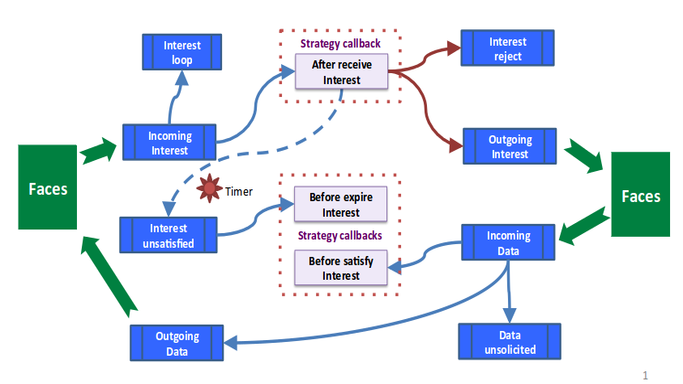
\includegraphics[height=3in, width=3.2in]{./Figures/Pipeline}
%			\caption{pipeline illustration of both programs working together}
%			\label{fig:not_congested_results1}
%		\end{figure} 



\begin{thebibliography}{99}

\bibitem{ndn}
NDN Named Data Networking project. [Online]. Available:
http://www.named-data.net/


\bibitem{NFD}
Named Data Networking Forwarding Daemon. [Online]. Available:
http://named-data.net/doc/NFD/current/


\bibitem{ndnsim}
NS-3 based Named Data Networking (NDN) simulator 
[Online]. Available:
http://ndnsim.net/

\bibitem{devguide}
Afanasyev, A., Shi, J., Zhang, B., Zhang, L., Moiseenko, I., Yu, Y., Fan, C. (2014). NFD developer’s guide. Technical Report NDN-0021, NDN.


\bibitem{ndncxx}
ndn-cxx: NDN C++ library with eXperimental eXtensions [Online]. Available:
https://named-data.net/doc/ndn-cxx/current/


\bibitem{docker}
Docker platform.
[Online]. Available:
https://www.docker.com/

\end{thebibliography}
  

\end{document}